\cotefile{43}
\scanpage{64}
% top product, with its lower identification
\[
\underbrace{\prod_{{\unsure{p|\mathfrak p}}_1\unsure{<|\backslash}p_2<\cdots<\text{\uline{\uuline{$p_n$}}}}
 A_{[p_1,p_2\unsure{-|,}p_n]}}_{{\unsure{\mathscr A|\mathcal A}}^{\unsure{n|u}}}
 \leftarrow \prod_{{\unsure{q|\mathfrak q}}_1<\cdots<q_{n-1}} A_{[q_1,\ldots,q_{n-1}]}
\]
\margin{\unsure{cosimplicial} ?!}
\[
p_1\supset p_2\supset\cdots\supset p_n
\]
\[
x_1\leq x_2\;\text{---}\;\leq x_n
\]
\figure{\begin{tikzpicture}[scale=.8]
\draw[<-] (0,0)--(3.4,-.3);
\draw (-.25,-.55)--(.05,.35) (.55,-.6)--(.75,.4) (2.7,-.65)--(3,.35);
\draw (5.3,1.25)--(5.35,1.05) (7.3,1.25)--(7.3,1.05);
\draw[->] (.2,.55)--(.7,.55); \draw (1.15,.55)--(1.4,.5) (2.3,.45)--(2.9,.45);
\end{tikzpicture}}
\[
A_{p,q}
\]
\figure{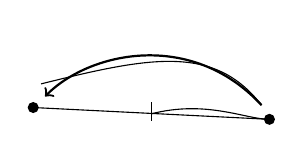
\begin{tikzpicture}
\fill (0,0) circle(2pt) (3,-.15) circle(2pt);
\draw (0,0)--(3,-.15); \draw (1.5,-.17)--(1.5,.07);
\draw[->,thick] (2.9,.03) .. controls (2,1) and (.7,.7) .. (.15,.14);
\draw (1.5,-.08) .. controls (2.2,.1) and (2.7,-.15) .. (3,-.15);
\draw (.1,.3) .. controls (1.5,.65) and (2.3,.8) .. (2.9,.03);
\end{tikzpicture}}
\[
\prod_{q<p} A_{[q,p]}\qquad \theta^2=0
\]
\figure{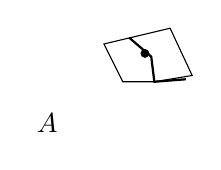
\begin{tikzpicture}[scale=.8]
\node at (-1.2,-.65) {$A$};
\draw (0,0)--(-.3,.6)--(.75,.85)--(1.1,.1)--(.5,0)--cycle;
\draw[thick] (.1,.7)--(.45,.4)--(.5,0)--(1,.04);
\fill (.35,.45) circle(2pt);
\end{tikzpicture}}
% middle, arrows and products
\diagram{\begin{tikzcd}[ampersand replacement=\&,column sep=large,row sep=large]
{}\& {\sum1_{q,p}} \arrow[l,bend right=12] \arrow[ddr,bend left=65] \& \\
{} \& {[p_1\supset\cdots\supset p_n]} \arrow[l] \arrow[d,"1_{qp}"] \arrow[dl,"{\unsure{\coprod}}_{q}1_{q,p_1}"'] \& \\
{\prod_q [q\supset p_1\supset\cdots\supset p_n]} \& {} \& {\prod_q[p_1\supset\cdots\supset p_n\supset q]}
\end{tikzcd}}
\figure{\begin{tikzpicture}
\draw[<-] (0,0)--(3.1,0);
\draw (0,.9) .. controls (0,.5) and (1,.6) .. (1.5,.7) .. controls (2,.9) and (2.2,.1) .. (3.2,.5);
\draw (1.2,2.1) .. controls (1,2.5) and (1.7,2.6) .. (2.1,2.4) .. controls (3,2.1) and (4,2.5) .. (4.2,1.9);
\draw[<-] (3.6,2)--(4.2,2);
\end{tikzpicture}}
\par\noindent\rule{\linewidth}{.4pt}
% lower notes
\[
A_{[p_1,\ldots,p_r]}
\]
\margin{$\unsure{\widehat A_p/p\widehat A_q|\widehat A_q/p\widehat A_q}$}
\unsure{anneau local} \unsure{muni} de $r$ topologies (\unsure{non adiques en général}) \unsure{différentes}, ${\unsure{T|\mathbb T|\Pi}}_1,\ldots,T_r$ (\unsure{pas nécessairement compatibles}) \unsure{métrisables} \deleted{\unsure{séparées}} et \unsure{complètes}.
\margin{$\widehat A_q$}
\figure{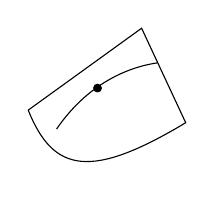
\begin{tikzpicture}[scale=.8]
\draw (0,.1)--(1.8,1.4)--(2.5,-.1) .. controls (1,-1) and (.4,-.9) .. (0,.1);
\draw (.45,-.2) .. controls (1,.6) and (1.7,.8) .. (2.05,.85);
\fill (1.1,.45) circle(2pt);
\end{tikzpicture}}
\unsure{Un} \unsure{germe} \unsure{filtré} \unsure{tend} vers $0$ pour $T_i$, \unsure{à} \unsure{fond} et \unsure{uniformément} \unsure{pour} \unsure{pour} $\forall$ voisinage de $0$ $V_{i+1}$ pour $T_{i+1}$,
% archive sheet number: 65
\scanpage{65}
% top, two brackets over the three symbols
\figure{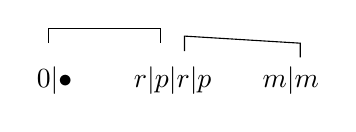
\begin{tikzpicture}[x=1cm,y=1cm]
\node at (0,0) {$\unsure{0|\bullet}$};
\node at (1.5,0) {$\unsure{r|p|\mathfrak r|\mathfrak p}$};
\node at (3,0) {$\unsure{m|\mathfrak m}$};
\draw (-.08,.48)--(-.08,.67)--(1.35,.67)--(1.35,.48);
\draw (1.65,.38)--(1.65,.57)--(3.12,.48)--(3.12,.3);
\end{tikzpicture}}
\[
\widehat A_r\otimes_A K\qquad \widehat{\widehat A\otimes A_r}
\]
\[
\deleted{\widehat{A/r^nA}\otimes A}\qquad \deleted{A_r}\qquad \deleted{A/r^nA}
\]
\[
A/m=\deleted{\unsure{k}} {\unsure{B|\mathscr B}}_0=L_0
\]
\[
\begin{aligned}
\widehat{A/r}&=B_1\subset L_1=\text{\unsure{anneau total des}}\\
&\qquad\text{\unsure{fractions de}}\quad\widehat{A/r}=B_1,\\
&=\unsure{\widehat{A/r}|\widehat A_r}\otimes_A A_r/rA_r
\end{aligned}
\]
\margin{$\varprojlim L_1$}
\figure{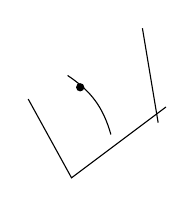
\begin{tikzpicture}
\draw (0,.7)--(.55,-.3)--(1.75,.6); \draw (1.45,1.6)--(1.65,.4);
\draw (.5,1) .. controls (.8,.8) and (.95,.6) .. (1.05,.25);
\fill (.66,.85) circle(1.5pt);
\end{tikzpicture}}
\figure{\begin{tikzpicture}[x=1cm,y=1cm]
\node at (0,0) {$A$};\node at (2,0) {${\unsure{p|\mathfrak p}}_1$};
\node at (2.75,0) {$\supset$};\node at (3.5,0) {$p_2$};
\node at (4.25,0) {$\supset$};\node at (5,0) {$\cdots$};
\node at (5.75,0) {$\supset$};\node at (6.5,0) {$p_n$};
\draw (2,.35)--(2,.52)--(3.25,.52)--(3.25,.35);
\draw (5.65,.35)--(5.65,.52)--(6.55,.52)--(6.55,.35);
\node at (2.65,.8) {$1$};\node at (6.1,.8) {$1$};
\end{tikzpicture}}
\[
A_{[p_1,p_2,\ldots,p_n]}
\]
\unsure{définition par récurrence sur} $n\geq1$

\margin{$A\unsure{\longrightarrow|-}\widehat A_p$ \unsure{anneau local complet}}
\[
A_{\unsure{\{p\}|[p]}}=\widehat A_p
\]
si $n=1$ ; c'est un \deleted{\unsure{filtre|fibré}} \inserted{\unsure{anneau}} local noeth. \inserted{\unsure{sur $A$}} et \unsure{complet} et une \unsure{algèbre} sur $A$.
\[
\begin{gathered}
A_{p,\unsure{q|\mathfrak q}}=\deleted{\unsure{\prod}}\varprojlim_n\widehat A_p\otimes_A A_q/q^nA_q
\qquad A_{[p_1\,\text{--}\,p_{n-1}]}\\
p\supset q\\
\widehat{A_p/qA_p}\quad\otimes
\end{gathered}
\]
\unsure{déjà défini}, c'est un \unsure{anneau} local \unsure{noethérien} \unsure{séparé} et \unsure{complet}, et une \unsure{algèbre} sur $A$.

\unsure{anneau semi-local complet} dont le \deleted{\unsure{corps}} \inserted{\unsure{anneau}} résiduel $\unsure{k|\kappa}(p,q)$ est l'anneau \unsure{tot.l|total} des fractions de
\[
\widehat{A_p/qA_p}=\widehat A_p/q\widehat A_p
\]
(\unsure{complété d'un anneau} local \unsure{intègre} noeth. de dim $1$)
% archive sheet number: 64
\scanpage{66}
\[
\unsure{\mathscr A|\mathcal A}\qquad \deleted{\theta^2=0}
\]
\[
A-\unsure{B|\mathscr B}
\]
\[
\theta_{\unsure{xx'|xu}}=\qquad\theta\deleted{\unsure{B}}
\]
\[
\theta^2=0\qquad\deleted{\unsure{A\theta\theta1|A\theta\theta_1}}
\]
\[
\unsure{\varphi|\phi}\qquad \pi_{x'}\theta\pi_x=\theta_{xx'}
\]
\figure{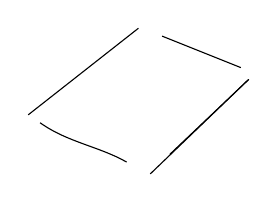
\begin{tikzpicture}
\draw (0,0)--(1.4,1.1) (1.7,1)--(2.7,.6) (2.8,.45)--(1.55,-.75) (.15,-.1)..controls(.5,-.35)and(.9,-.4)..(1.25,-.6);
\draw (2.8,.45)--(1.8,-.5);
\end{tikzpicture}}
\[
\deleted{x_1\unsure{\in|<}x_2\unsure{\in|<}x}
\qquad x_1\geq x_2\geq x_3\;\text{--}\;\geq\underbrace{x_n\geq x_{n+1}}\geq x_{\unsure{n+m|n+2}}
\]
\[
\theta_{x_1,\unsure{x_2|x_n}}\quad\theta
\]
\[
\pi_{x_{\unsure{m|n+m}}}\theta\;\text{--}\;\pi_{x_{n+2}}\theta\pi_{x_{n+1}}
\underbrace{\varphi_{x_n x_{n+1}}\pi_{x_n}}
\underbrace{\theta\cdots\pi_{x_3}\theta\pi_{x_2}\theta\pi_{x_1}}
\]
\figure{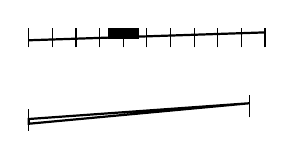
\begin{tikzpicture}
\draw[thick] (0,1)--(3,1.1);
\foreach \x in {0,.3,.6,.9,1.2,1.5,1.8,2.1,2.4,2.7,3}{\draw (\x,.91)--(\x,1.15);}
\fill (1,1.02) rectangle (1.4,1.16);
\draw[thick] (0,0)--(2.8,.2)--(0,-.06)--cycle;
\draw (0,-.15)--(0,.13) (2.8,.02)--(2.8,.3);
\end{tikzpicture}}
\[
\unsure{\varphi_n|\varphi_x}\qquad\unsure{\varphi_{x'}|\theta_{x'}}
\]
\figure{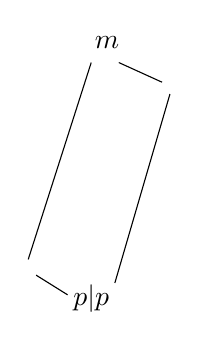
\begin{tikzpicture}
\draw (0,0)--(.8,2.5) (1.15,2.5)--(1.7,2.25) (1.8,2.1)--(1.1,-.3) (.1,-.2)--(.5,-.45);
\node at (1,2.75) {$\unsure{m}$}; \node at (.8,-.5) {$\unsure{p|\mathfrak p}$};
\end{tikzpicture}}
\[
\left\{\begin{aligned}
&\theta\quad A\text{-\unsure{linéaire}}\\
&\theta^2=0\\
&\theta\text{ de degré }1
\end{aligned}\right.
\qquad\theta
\]
\diagram{\begin{tikzcd}[ampersand replacement=\&,row sep=small,column sep=small]
\bullet \arrow[dd,bend right=30] \&\&\\
\bullet\arrow[d] \& {}\arrow[r,dash] \&\bullet\arrow[d]\\
\bullet \& {}\arrow[l] \&\bullet \&\bullet\arrow[l]\arrow[ll,bend left=35]
\end{tikzcd}}
\figure{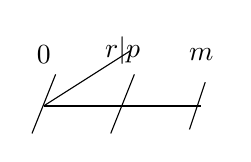
\begin{tikzpicture}
\draw[thick] (0,0)--(2,0);
\draw (-.15,-.35)--(.15,.4) (.85,-.35)--(1.15,.4) (1.85,-.3)--(2.05,.3);
\draw (0,0)--(1.1,.7); \node at (0,.65) {$0$};\node at (1,.7) {$\unsure{r|p}$};\node at (2,.65) {$\unsure{m}$};
\end{tikzpicture}}
\margin{$\operatorname{Hom}$}
\[
\unsure{\mathscr H|\mathcal H}
\]
\deleted{anneau gradué topologique,}

$\mathscr A^*$ \deleted{$\unsure{\mathscr H|\mathscr A}$} \unsure{algèbre topologique} \inserted{(\unsure{séparée, complète})} \unsure{graduée} sur $A$, à degrés $\geq0$, avec
\[
\left\{\begin{aligned}
\mathscr A_0^{\unsure{0|\circ}}&=\deleted{\unsure{\simeq}}\prod_{x\in X}\widehat{\unsure{\mathscr O|\mathcal O}}_x
\quad\text{d'où des}\quad\pi_x\in\mathscr A_0\quad(x\in\unsure{X|\mathscr X})\\
&\text{(\unsure{isom d'$A$-algèbres topologiques})}\\
\theta&\in\mathscr A_1^1,\quad\text{avec}\quad\underline{\theta^2=0},\quad
\underline{\pi_{x'}\theta\pi_x=0\quad\deleted{\unsure{x}}\quad\text{si $x'$ ne \unsure{précède} pas $x$}}
\end{aligned}\right.
\]
$\mathscr A$ libre pour ces propriétés \text{------}
% archive sheet number: 65
\scanpage{67}
\deleted{$\operatorname{Hom}$}
\[
\deleted{\unsure{H^*(A)}=\varinjlim}
\]
\[
\underbrace{\operatorname{Hom}(K\deleted{\unsure{xy|(x,y)}},K)}_{\substack{A\text{-\unsure{algèbre graduée}}\\\text{\unsure{pour la composition}}\\\text{\unsure{des hom}}}}
=\prod_x\operatorname{Hom}(K(x),K)\supset\prod_x\coprod_y\operatorname{Hom}(K(x),K(y))
\]
\margin{$K(x)\longrightarrow\coprod_{x'}K(x')$}
\[
\prod_x\operatorname{Hom}(K(x),K(x))
\]
\[
\prod_x\qquad\deleted{\operatorname{Hom}^{0}(K}
\]
\[
\operatorname{Hom}^{\unsure{0}}(K,K)^0=\prod_x\widehat{\unsure{\mathscr O|\mathcal O}}_x
\quad\text{\unsure{engendrés}}\quad\text{\textcircled{$\pi_x$}}
\]
\[
\theta\in\operatorname{Hom}(K,K)^1=\prod_x\operatorname{Hom}\left(K(x),\coprod_{\substack{\underline{x'}\,\text{\unsure{prime|précède}}\,x}}K_{x'}\right)
\simeq\prod_{\substack{\text{\unsure{restreint}}\\x'\,\text{\unsure{prime|précède}}\,x\\\deleted{\unsure{2?}}}}\widehat{\mathscr O}_{x,x'}
\]
\margin{(la différentielle)}
\[
\deleted{\unsure{\pi_x\theta}}\quad\pi_{x'}\theta\pi_x\quad.\quad
\deleted{\unsure{\widehat{\mathscr O}_x\theta\widehat{\mathscr O}_{x'}}}
\]
\[
\widehat{\mathscr O}_{x,x'}
\]
\diagram{\begin{tikzcd}[ampersand replacement=\&]
\mathscr O_{x'}\arrow[r,no head]\arrow[d,equal]\&\mathscr O_x\arrow[d,equal]\\
A\&A_{\unsure{p|\mathfrak p}}
\end{tikzcd}}
\figure{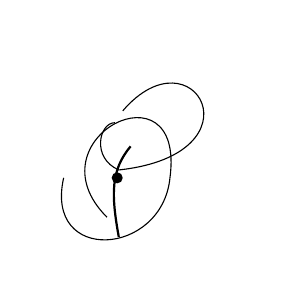
\begin{tikzpicture}
\draw (0,0) .. controls (-1,1) and (1,2) .. (.8,.5) .. controls (.7,-.5) and (-.8,-.6) .. (-.55,.5);
\draw (.2,1.35) .. controls (1.1,2.4) and (2,.8) .. (.15,.6) .. controls (-.2,.75) and (-.1,1.2) .. (.1,1.2);
\draw[thick] (.15,-.25)..controls(.05,.3)and(.05,.6)..(.3,.9);\fill (.13,.5) circle(2pt);
\end{tikzpicture}}
\[
\underbrace{\sum{\unsure{\varphi|\phi}}_{x'}\theta\varphi_x}\qquad\pi_{x'}
\]
\[
A_p\rightsquigarrow\overline I_A\qquad\widehat A\otimes_A A_p/p^nA_p
\]
\[
D(A_p/p^nA_p)-\overline I_{A_p/p^nA_p}\qquad
\widehat A\otimes_A\widehat A_p\qquad\widehat{A/p}
\]
\[
\unsure{\delta|\Gamma|\mathscr D|\mathscr T}(\unsure{uv|u\sigma|\mu v|\mu\sigma})=\qquad A_{p,p'}
\]
\[
[\theta,x]\qquad\operatorname{Hom}(K,K)
\]
\[
\{\theta,\unsure{u|x}\}=\theta\unsure{u|x}+(-1)^{\deg\theta\deg\unsure{u|x}}u\theta
=\theta u+(-1)^{\deg u}u\theta
\]
$[$\unsure{si} $\deg u=0$, $\deg\theta=1$, \unsure{on a} $\theta u-u\theta$
% archive sheet number: 66
\scanpage{68}
\[
K(x)\longrightarrow\coprod_y K(y)
\]
\diagram{$\left\{\vcenter{\hbox{\begin{tikzcd}[ampersand replacement=\&,row sep=small]
x\arrow[d]\\x'\arrow[d]\\x''
\end{tikzcd}}}\right.$}
\diagram{\begin{tikzcd}[ampersand replacement=\&,column sep=large]
K(x)\arrow[r]\&\displaystyle\coprod_{x'\,\text{précède}\,x}K(x')\arrow[d]\\
\&\displaystyle\coprod_{x''\,\text{\unsure{biprécède}}\,x}K(x'')
\end{tikzcd}}
\margin{$K(x)\unsure{\longrightarrow|-}\displaystyle\prod_{x'\,\text{\unsure{pré}}}$}
\[
\underbrace{K(x)\longrightarrow\coprod_{\substack{x'\\\text{\unsure{les intermédiaires}}\\\text{entre }x\text{ et }x''}}K(x')\longrightarrow K(x'')}_{\text{nul}}
\]
\[
\deleted{\operatorname{Hom}(K(x),K(y))}
\]
\[
\begin{aligned}
\operatorname{Hom}(K,K)&=\prod_x\operatorname{Hom}(K(x),K)\\
&=\prod_x\prod_y^{\text{\unsure{restreint}}}\underbrace{\operatorname{Hom}(K(x),K(y))}_{H(x,y)}
\end{aligned}
\]
$H(x,x)$ \unsure{un anneau}
\[
H(x\qquad K\rightsquigarrow I
\]
\figure{\begin{tikzpicture}
\draw[->] (0,0)--(4,.3);\foreach \x in {0,.8,1.6,2.4,3.2}{\draw (\x,-.05+.075*\x)--(\x,.08+.075*\x);}
\draw[->,dashed] (0,.1)..controls(1.4,1.4)and(3.6,1)..(4.1,.3);
\end{tikzpicture}}
\[
\operatorname{Hom}(K,
\]
\diagram{\begin{tikzcd}[ampersand replacement=\&,row sep=small,column sep=large]
\unsure{q|\varphi}\mid\arrow[r,dash]\&{}\arrow[rr,dash,very thick]\&{}\&K(y')\arrow[d]\\
\&K(x)\arrow[u]\arrow[urr,shift left]\arrow[urr,shift right]\arrow[rr,dash]\arrow[dr]\&{}\&K(y)\\
\&{}\&K(x')\arrow[ur]\&{}
\end{tikzcd}}
\figure{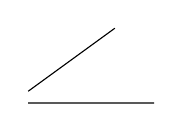
\begin{tikzpicture}\draw (0,0)--(1.1,.8) (0,-.15)--(1.6,-.15);\end{tikzpicture}}
\[
\unsure{q|\mathfrak q}\supset\unsure{p|\mathfrak p}\qquad K(p)\longrightarrow I
\]
\figure{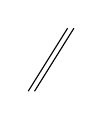
\begin{tikzpicture}\draw (0,0)--(.5,.8) (.08,0)--(.58,.8);\end{tikzpicture}}
\[
\operatorname{Hom}(K,D(A))
\]
\inserted{\unsure{un cas particulier}}
\diagram{\begin{tikzcd}[ampersand replacement=\&,column sep=large,row sep=small]
\&\&*\arrow[d,"d'_{\unsure{g|q}}"]\\
\bullet\arrow[urr,Rightarrow]\arrow[rr,Rightarrow]\arrow[dr,"d"']\&\&\deleted{\unsure{\theta}}\arrow[dr,"d'"]\\
\&\bullet\arrow[rr]\&\&\bullet
\end{tikzcd}}
\diagram{\begin{tikzcd}[ampersand replacement=\&,column sep=small,row sep=small]
\&{}\arrow[dr,"d"]\&\&\&\\
\&\&{}\arrow[dr,"d"]\&\&\\
\bullet\arrow[uur,"3"]\arrow[urr,"2"]\arrow[rrr,"1"]\arrow[dr,"d"']\&\&\&\bullet\arrow[dr,"d"]\&\\
\&{}\arrow[uur,"3"]\arrow[urr,"2"]\arrow[rrr,"1"']\arrow[dr,"d"']\&\&\&{}\\
\&\&{}\arrow[uur,"3"]\arrow[urr,"2"']\arrow[dr,"d"']\&\&\\
\&\&\&\bullet\arrow[uur,"3"']\&
\end{tikzcd}}
\figure{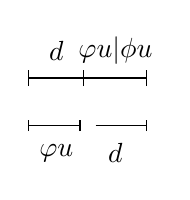
\begin{tikzpicture}
\draw[thick] (0,.6)--(1.5,.6); \foreach \x in {0,.7,1.5}{\draw (\x,.5)--(\x,.7);}
\node at (.35,.95) {$d$};\node at (1.1,.95) {$\unsure{\varphi u|\phi u}$};
\draw (0,0)--(.65,0) (.85,0)--(1.5,0);\draw (0,-.07)--(0,.07) (.65,-.07)--(.65,.07) (1.5,-.07)--(1.5,.07);
\node at (.35,-.35) {$\unsure{\varphi u}$};\node at (1.1,-.35) {$d$};
\end{tikzpicture}}
\figure{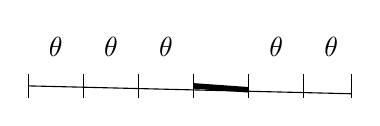
\begin{tikzpicture}
\draw (0,0)--(4.1,-.1);\foreach \x in {0,.7,1.4,2.1,2.8,3.5,4.1}{\draw (\x,-.15)--(\x,.15);}
\draw[line width=2pt] (2.1,0)--(2.8,-.05);
\foreach \x in {.35,1.05,1.75,3.15,3.85}{\node at (\x,.5) {$\theta$};}
\end{tikzpicture}}
\figure{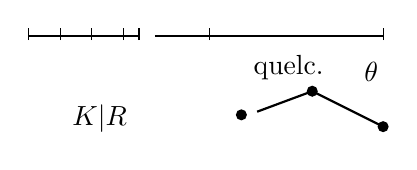
\begin{tikzpicture}
\draw[thick] (0,1)--(1.4,1) (1.6,1)--(4.5,1);\foreach \x in {0,.4,.8,1.2,1.4,2.3,4.5}{\draw (\x,.95)--(\x,1.1);}
\node at (.9,-.05) {$\unsure{\mathscr K|\mathscr R}$};
\fill (2.7,0) circle(2pt) (3.6,.3) circle(2pt) (4.5,-.15) circle(2pt);
\draw[thick] (2.9,.04)--(3.6,.3)--(4.5,-.15);
\node at (3.3,.6) {\unsure{quelc.}};\node at (4.35,.55) {$\theta$};
\end{tikzpicture}}
% archive sheet number: 67
\scanpage{69}
\diagram{\begin{tikzcd}[ampersand replacement=\&,column sep=large]
\&K(x)\arrow[r,very thick,"x\geq y"]\&K(y)\arrow[dr]\\
K(x')\arrow[ur]\arrow[rrr,no head]\&\&\&K(y')
\end{tikzcd}}
\[
x'\geq\underbrace{x\geq y}\geq y'
\]
\[
H(x,y)\longrightarrow H(x',y')
\]
\unsure{chaque fois qu'on se donne un chemin saturé} \unsure{joignant} $x$ à $x'$ et un \unsure{autre} joignant $y'$ à $y$.
\[
y'\rightsquigarrow\longleftrightarrow x\rightsquigarrow x'
\]
\unsure{Si} : \unsure{tout} \unsure{chemin|chaîne} \unsure{saturée|saturé} $s$ joignant $x$ à $y$, on associe $H_s=H(x,y)$, alors si $s\leq s'$, alors $H_s\longrightarrow H_{s'}$ ; \deleted{d'ailleurs $H_{\unsure{s'|s}}$ est \unsure{engendré} par les images des $H_{s'}$, \unsure{ou|où} $s'\leq s$, $s'$ \uline{\unsure{contigu}} à $s$}
\figure{\begin{tikzpicture}
\draw[line width=2pt] (0,1.4)--(1.2,1.4);\draw (.6,1.3)--(.6,1.55);\draw(0,1.2)--(.55,1.2);\fill(0,1.4)circle(2pt)(1.2,1.4)circle(2pt);
\draw (5,1.4)--(8,1.6);\fill (4.8,1.4)circle(1.5pt)(8,1.6)circle(2pt);
\draw (0,0)--(4,.03);\draw (0,-.12)--(0,.12) (.6,-.13)--(.6,.15);\fill (4,.03)circle(2pt);
\end{tikzpicture}}
\[
H_s\quad s\text{ de longueur }0\qquad
H_s\quad s\text{ de longueur }1
\]
\figure{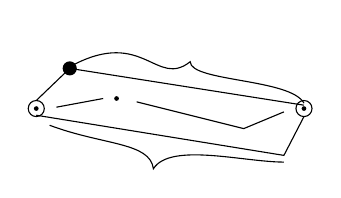
\begin{tikzpicture}[scale=.85]
\draw (0,0)circle(.12);\fill(0,0)circle(1pt)(.5,.6)circle(3pt);\draw (4,0)circle(.12);\fill(4,0)circle(1pt);
\draw (0,.12)--(.5,.6)--(4,.05) (0,-.1)--(3.7,-.7)--(4,-.12);
\draw (.3,.02)--(1,.15);\fill(1.2,.15)circle(1pt);\draw(1.5,.1)--(3.1,-.3)--(3.7,-.05);
\draw (.55,.65)..controls(1.6,1.2)and(1.8,.3)..(2.3,.7)..controls(2.3,.4)and(3.8,.45)..(4,.08);
\draw (.2,-.25)..controls(1,-.55)and(1.7,-.5)..(1.75,-.9)..controls(2,-.5)and(3.1,-.8)..(3.7,-.8);
\end{tikzpicture}}
\figure{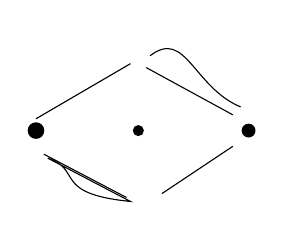
\begin{tikzpicture}
\fill(0,0)circle(3pt)(1.3,0)circle(2pt)(2.7,0)circle(2.5pt);
\draw (0,.15)--(1.2,.85) (1.4,.8)--(2.5,.2) (2.5,-.2)--(1.6,-.8) (.1,-.3)--(1.15,-.85);
\draw (1.45,.95)..controls(1.9,1.3)and(2,.55)..(2.6,.3);
\draw (.15,-.35)..controls(.6,-.5)and(.2,-.8)..(1.2,-.9)--(.15,-.35);
\end{tikzpicture}}
\diagram{\begin{tikzcd}[ampersand replacement=\&]
\left(\displaystyle\coprod_{s\in C_2(x,y)}H_s\right)\left(\displaystyle\coprod_{t\in C_{\unsure{1|2}}(x,y)}H_t\right)\\
H_{s\in C_0(x,y)}\arrow[u]
\end{tikzcd}}
\[
K_n=\coprod H_s\qquad\prod_x H\left(x,\coprod y\right)
\]
\[
\prod_x\prod_{y\,\text{\unsure{loc}}}H(x,y)
\]
\diagram{\begin{tikzcd}[ampersand replacement=\&,column sep=tiny]
{}\arrow[r,very thick]\arrow[rrr,dashed,bend right]\&{}\arrow[r]\&{}\arrow[r]\&{}\arrow[r]\&{}\arrow[r]\&{}\arrow[r]\&{}
\end{tikzcd}}
$I$ \unsure{ensemble ordonné} ``discret'' \unsure{au sens large}

$\widetilde I$ \unsure{catégorie des flèches composées}

$K$ \deleted{$\unsure{K}$} \unsure{foncteur} de $\widetilde I$ dans $C$
% archive sheet number: 68
\scanpage{70}
Jacobiennes locales
% archive sheet number: 69
\scanpage{71}
\margin{\figure{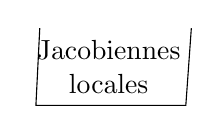
\begin{tikzpicture}[x=.7cm,y=.7cm]
\node[align=center] at (1.1,.65) {Jacobiennes\\locales};
\draw (-.15,1.35)--(-.22,-.05)--(2.5,-.05)--(2.6,1.35);
\end{tikzpicture}}}
% loop at upper left; possibly a physical paperclip
\figure{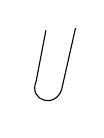
\begin{tikzpicture}[scale=.5]\draw (0,1.6)--(-.25,.3)..controls(-.45,-.2)and(.25,-.4)..(.4,.1)--(.75,1.65);\end{tikzpicture}}
\unsure{Tout dépend de quelle théorie}. \unsure{Il y en a plusieurs} :

I) Théorie \unsure{Čechiste} pour la topologie de Zariski.

(Celle où le $H^1$ \unsure{classifie} les \deleted{\unsure{ses}} fibrés principaux \uline{loc.} \uline{triviaux}). Il n'y a \inserted{\unsure{à priori}} de \unsure{suite exacte de coh.} pour $0-G'-G-G''-0$ \uline{que} si la suite est \unsure{loc triviale}.

Si $X=\unsure{\operatorname{Spec}|\operatorname{Sp}}(A)$ est le spectre d'un anneau \uline{local} on aura
\[
\begin{aligned}
H^i(X,G)&=0&&\text{si }i>0\\
H^i(X-a,G)&=0&&\text{si }i\geq\dim A\quad\deleted{\unsure{\dim(X-a)+1}}
\end{aligned}
\]
\inserted{[car $\dim(X-a)\leq\dim A-1$]}

d'où
\[
0-H^0(X/X-a,G)-H^0(X,\unsure{G})-H^0(X-a,G)-H^1(X/X-a,G)\longrightarrow0
\]
\[
H^i(X/X-a,G)\xleftarrow[\sim]{\unsure{\partial|\delta}}H^{i-1}(X-a,G)\qquad(i\unsure{\geq|>}2)
\]
\inserted{[\uline{c'est nul si $i>\dim A$\deleted{$\unsure{1}$}}]}

On supposera $A$ \uline{régulier}.
\[
\text{a)}\quad H_A^0(G)=\left\{\begin{aligned}
&G(A)=G(K)&&\text{si }\dim A=0\\
&0&&\text{si }\dim A>0
\end{aligned}\right.
\]
Le foncteur $H_A^0(G)$ est \unsure{exact} pour les suites \deleted{\unsure{split exactes}} \inserted{exactes} loc. triviales
\margin{\deleted{\illegible{3}} \deleted{(\unsure{distinguer cas $A$ abélien} \illegible{2} \unsure{et le cas $G$ affine})}}
\[
\text{b)}\quad H_A^1(G)=\left\{\begin{aligned}
&0&&\text{si }\dim A\neq1\\
&G(K)/G(A)&&\text{si }\dim A=1
\end{aligned}\right.
\]
Ce foncteur $H_A^1(G)$ est \unsure{exact} pour les suites exactes loc. triviales
% slanted
\margin{\unsure{Prouve que} si $\dim A=1$, ${\unsure{J|\mathscr J}}_{A/k}$ est \uline{connexe} \unsure{sans composante abélienne} (car $H_A^1(G)$ est nul pour $G$ \unsure{propre ou} $G$ discret)}
\margin{\deleted{$\unsure{G_{\mathrm{Ab}}}$}\deleted{\illegible{3}}}
\[
\text{c)}\quad H_A^2(G)=H^1(X-a,G)=\left\{\begin{aligned}
&0\text{ si }\dim A\neq2\\
&\text{\unsure{en tous cas ne dépend que de}}\\
&\text{\unsure{la composante connexe}}\\
&\text{\unsure{unipotente} de }G.
\end{aligned}\right.
\]
% archive sheet number: 70
\scanpage{72}
% writing upside down in the supplied scan; two long cancellation strokes through the draft
\[
\deleted{\text{a)}\quad H_A^0(G)=\operatorname{Ker}\left[G(\unsure{\operatorname{Spec}|\operatorname{Sp}}(A))\longrightarrow G(\operatorname{Spec}(A)-a)\right]=\left\{\begin{aligned}G(A)&\quad\text{si }\dim A=0\\0&\quad\text{si }\dim A\neq0\end{aligned}\right.}
\]
\deleted{\unsure{b}}

\deleted{Si $\dim A=0$, le foncteur $H_A^0(G)$ est exact pour les suites exactes \unsure{qui sont} loc. triviales.}
\[
\deleted{\text{b)}\quad H_A^1(G)=\operatorname{Coker}\left(G(\operatorname{Spec}(A))\longrightarrow G(\operatorname{Spec}(A)-a)\right)=\left\{\begin{aligned}G(K)/G(A)&\quad\text{si }\dim A=1\\0&\quad\text{si }\dim A\neq1\end{aligned}\right.}
\]
\[
\deleted{\text{c)}\quad H_A^{?}(G)=H^1_{?}(\operatorname{Spec}(A)-a,G)}
\]
\deleted{il faut choisir sa \unsure{théorie cohomologique} (fibrés loc. triviaux, \unsure{strictement isotriviaux}, \unsure{isobirationnels}). \unsure{On trouve} :}
% archive sheet number: 71
\scanpage{73}
\margin{Si $\dim A=0$ ou $1$, il n'y a \unsure{rien à prouver}, \unsure{on peut supposer|supposons} $\dim A\geq2$}
Soit ${\unsure{\mathscr H|\mathcal H}}^1$ le \deleted{\unsure{gr.}} \unsure{ens.} des classes de fibrés principaux homogènes (\unsure{triv} par extension fid. plat quasi compacte de la base). On aura $H^1(X-a,G)\subset\mathscr H^1(X-a,G)$, qui lui est \unsure{partie} d'un foncteur coh. en $G$.

On a si \deleted{$\unsure{\dim A=0}$} $G$ est \deleted{\unsure{une variété abélienne}} \inserted{\uline{propre} sur $k$}
\[
H^1(X-a,G)\deleted{=\unsure{H^1(X,G)}}=0\qquad(\text{loc trivial}=\text{trivial}),
\]
\unsure{donc on prouve|donc on prouvera} $\unsure{\forall|\text{tt}}$ élément \unsure{de|d'un} $H^1(X-a,G)$ \unsure{provient} de $\mathscr H^1(X-a,L)$, $L$ le ss-gpe linéaire \inserted{\uline{connexe}}.

Or pour un gpe linéaire \inserted{connexe}, on sait que \deleted{$H^1=\mathscr H^1$} $H^1(G)=\mathscr H^1(G)$, donc on \deleted{\unsure{est}} aura
\[
H^1(X-a,G)=\deleted{H^1(X-a,L)}\operatorname{Im}\bigl(H^1(X-a,L)\longrightarrow H^1(X-a,G)\bigr)
\]
\[
\operatorname{Im}\bigl(\mathscr H^1(X-a,L)\longrightarrow\mathscr H^1(X-a,G)\bigr)
=H^1(X-a,L)/\operatorname{Im}H^0(X-a,G/L)
\]
Or $H^0(X-a,G/L)=H^0(X,G/L)$ qui \unsure{s'envoie} dans $H^1(X,L)=0$, donc $\uline{\ensuremath{H^1(X-a,G)}}=\uline{\ensuremath{H^1(X-a,L)}}$.

D'ailleurs, comme $X$ est factoriel, $H^1(X-a,G_m)=0$ d'où $H^1(X-a,L)=H^1(X-a,U)$, $U$ le \unsure{gpe} unipotent. Cette dernière se \unsure{dévisse} par les $H^1(X-a,G_a)$, qui sont nuls si $\dim A>2$, mais \unsure{non} \unsure{pour} \deleted{\unsure{si}} $\dim A=2$.

\[
\text{d)}\quad H_A^{\unsure{3}}(G)=H^2(X-a,G)
\]
De façon générale, on a \deleted{$H^i(X-a,G)=$} une suite exacte de faisceaux
\[
0\longrightarrow\underline{\unsure{\mathscr O|O}}_X(G)\unsure{\mathbin{\text{---}}|\longrightarrow}\underline{\unsure{\mathscr R|R}}_X(G)\mathbin{\text{---}}\underline{\unsure{\mathscr D|D}}_X(G)\mathbin{\text{---}}0
\]
d'où, puisque $\underline{\mathscr R}_X(G)$ est flasque
\[
H^i(\underline{\mathscr O}_X(G))=H^{i-1}(\underline{\mathscr D}_X(G))\quad\text{si }i\geq2
\]
% archive sheet number: 72
\scanpage{74}
D'autre part, \deleted{\unsure{comme}} si $L$ est la partie linéaire de $G$, on a \deleted{$\unsure{H}$} $\underline{\unsure{\mathscr D|D}}_X(G)\simeq\underline{\mathscr D}_X(L)$, d'où
\[
H^i(\unsure{X|A}-a,G)\simeq H^i(X-a,L)\qquad(i\geq2,\text{ et }=\text{ on a vu pour }i\geq1)
\]
On sait par \unsure{là|l'a.} $H^i(X-a,G_m)=0$ puisque $X$ est factoriel, donc on aura $=$
\[
H^i(X-a,G)=H^i(X-a,U)\qquad(i\geq1)
\]
\deleted{\unsure{C'est}} D'ailleurs \unsure{on a}
\[
H^i(X-a,G_a)=0\qquad\text{si }i\neq\dim A-1
\]
donc
\[
H^i(X-a,U)=0\qquad\text{si }i\neq\dim A-1
\]
\unsure{Ceci achève de prouver ce qu'on veut|Ceci achève de prouver ce qui précède}.

\unsure{Noter aussi} $H_A^i(G)\xrightarrow{\sim}H_{\widehat A}^i(G)$ : rien ne change en \unsure{remplaçant} $A$ par $\widehat A$.
% archive sheet number: 73
\scanpage{75}
Jacobienne locale \inserted{\unsure{relative}} d'une localité \inserted{(régulière)} $A$ sur un corps $k$

$J_{A/k}$ est défini par le foncteur $\operatorname{Hom}_{k\text{-grp}}(J_{A/k},G)$ en $G$ (grp. \inserted{loc.} de type fini sur $k$) on doit avoir
\[
\operatorname{Hom}_{k\text{-}\unsure{gr|grp}}(J_{A/k},G)\simeq H_A^i(G)\qquad i=\dim A
\]
% slanted, upper left
\margin{Le foncteur en $G$ est \unsure{représentable}, \unsure{grâce au fait que} $H_A^j(G)=0$ si $j\unsure{<|\leq}i$ \unsure{lorsque|dès que} $A$ est \uuline{régulier}.}
$H_A^i$ est le foncteur cohomologique de localisation pour l'anneau local $A$ [$\text{de }\unsure{\operatorname{Spec}|\operatorname{Sp}}(A):\operatorname{Spec}(A)-{\unsure{m|\mathfrak m}}_A$], foncteur qui est défini à priori sur les faisceaux de Weil sur $\operatorname{Spec}(A)$. On a
% slanted, middle left
\margin{\unsure{Tous les} $J_{A/k}$ \unsure{sont des} proalgébriques \uline{\unsure{simples|stricts}} sur $k$.}
\[
\begin{aligned}
H_A^0(G)&=G(K)&&\text{si }A=K\text{ de dim }0\\
H_A^1(G)&=G(K)/G(A)&&\text{si }A\text{ de dim }1,\text{ de corps de fractions }K\\
H_A^i(G)&=H^{i-1}(\operatorname{Spec}(A)-m_A,G)&&\text{si }A\text{ de dim}\geq2
\end{aligned}
\]
\unsure{Je trouve|Je résume} :

\noindent a) $J_{K/k}$ est une \uline{extension de} $\mathbb Z_{(k)}$ (qui correspond au foncteur $G\longmapsto G(k)$) par un groupe connexe, qui en général a \uline{une partie abélienne} (c'est le \unsure{Albanese} de $K/k$), \uline{une partie multiplicative} \inserted{$M$}, en plus de la partie unipotente \inserted{$U$}.
% slanted, right; marginal leader, relative geometry only
\figure{\begin{tikzpicture}[x=1cm,y=1cm]
\fill (0.12,1.5) circle (0.025);
\draw (0.12,1.5) .. controls (-0.2,1.25) and (0.2,0.3) .. (0.55,-0.7) .. controls (0.68,-1.05) and (0.68,-1.5) .. (0.38,-1.52);
\end{tikzpicture}}
\margin{\unsure{Ces} \deleted{\unsure{J}} J sont \unsure{rel.t|relt.} projectifs pour les \unsure{ext.|cat.} \unsure{qui sont des} fibrés loc. triv.}
\inserted{$J_{K/k}$ \unsure{n'est pas projectif en général, mais son} $\operatorname{Ext}^1$ \unsure{avec un groupe} \uline{linéaire} \uline{connexe} est \unsure{tjrs|toujours} \unsure{trivial}.}
% slanted, lower left, first note
\margin{$\unsure{D^{(M)}|D(M)}$. N.B. $\operatorname{Hom}_{k\text{-grp}}(M,G_m)=\deleted{\unsure{K^*/k^*}}=$ grp des diviseurs \deleted{\unsure{de} \illegible{2}} \unsure{alg. équiv. à} $0$ (sur un modèle \unsure{régulier}).}
% slanted, lower left, second note
\margin{$\operatorname{Hom}(U,G_a)=K/k$ \deleted{\unsure{différent.} \illegible{3} \unsure{triv.}} \unsure{mais les} \unsure{mêmes} \unsure{sur|en} ${\unsure{\mathscr F|F}}_{\unsure{n-1|i-1}}(\unsure{k_0|k.})$ \unsure{et|de}.}

\noindent b) Si $A$ est de dim $1$, $J_{A/k}$ \uline{connexe}, \uline{linéaire} (i.e. plus de partie abélienne) mais \unsure{elle a} \deleted{\unsure{le plus souvent|la plus souvent}} une \deleted{\unsure{grosse}} partie multiplicative \inserted{$M\simeq G_m$}
% archive sheet number: 74
\scanpage{76}
De plus, $J_{A/k}$ est \uline{projectif} \uline{relativement aux suites exactes loc. triviales}.
\inserted{i.e. son $\uline{\operatorname{Ext}^1}$ \unsure{avec} \uline{un \unsure{grpe|gpe} \unsure{lin.} connexe est $0$}.}

\noindent c) Si $\dim A\geq2$, alors $J_{A/k}$ est \uline{connexe}, \uline{unipotent} (i.e. plus de partie abélienne ni multiplicative) et de plus \uline{projectif} (car le foncteur \unsure{qu'elle|qu'il} représente est exact\inserted{)}\deleted{, comme pour $\dim A=1$)}
\figure{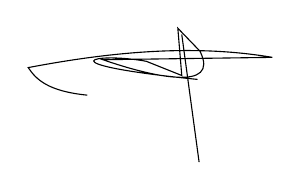
\begin{tikzpicture}[x=1cm,y=1cm]
\draw (0,0) .. controls (-.5,.05) and (-.65,.2) .. (-.75,.35) .. controls (.3,.55) and (1.35,.65) .. (2.35,.48) --(.2,.45) .. controls (.8,.24) and (1.7,.03) .. (1.43,.56) --(1.15,.85) --(1.2,.25) --(.75,.43) .. controls (.1,.55) and (-.6,.4) .. (1.4,.2);
\draw (1.2,.77)--(1.42,-.85);
\end{tikzpicture}}
% archive sheet number: 75
\scanpage{77}
II Cohomologie de Weil \unsure{\ldots} [\unsure{semble marcher moins bien}\ldots]

Il n'est plus vrai en général que \inserted{\unsure{Supposons} $A$ \uline{\unsure{hensél.}}}
\[
H^i(A,G)=0\qquad\text{si }i>0.
\]
\deleted{\unsure{Pour}} Si $G$ est $k$-\uline{\unsure{simple|ample}}, alors $H^i(A,G)=H^i(L,G)$ \inserted{si $i>0$}, $L$ étant le corps résiduel, et \deleted{si $i>0$} on a
\[
H^i(L,G)=H^i(L,G/\unsure{\mathscr L|\alpha})
\]
où $\mathscr L$ est le plus grand ss-gpe linéaire connexe de $G$.
\deleted{$\unsure{H_A}$ \unsure{ne serait pas} \illegible{2}}
\deleted{$\unsure{H_A}$ \unsure{ce qui est} \illegible{2}}

\deleted{$H^1(X/X-a,G)\unsure{-|\longrightarrow}H^1(X,G)$ \unsure{à déterminer à travers les}}
\deleted{Si $\dim A=0$, rien de nouveau.}
\deleted{Si $\dim A=1$, on a $H^1_{\unsure{l.t.|l.tr.}}(X,G)$, \unsure{donc est nul, d'où on aura}}
\[
\deleted{H^1_{\unsure{K|A}}(G)=\operatorname{Coker}(H^0(X)\unsure{-|\longrightarrow}H^0(X-a))}
\]

Si $\dim A=0$, rien de nouveau.

Si $\dim A\geq1$, alors $H^1(X/X-a,G)$ est extension de $\operatorname{Ker}(H^1(X,\unsure{G})-H^1(X-a,G))$ par $G(K)/G(A)$.

\inserted{Or} \deleted{\unsure{on a}}
\[
\operatorname{Ker}(H^1(X,G)\longrightarrow H^1(X-a,G))=0
\]
% lower-left marginal diagram
\margin{\diagram{\begin{tikzcd}[ampersand replacement=\&,column sep=small,row sep=small]
0\arrow[d]\&\\
H^1(X,G)\arrow[r]\arrow[d]\&H^1(X-a,G)\arrow[d]\\
H^1(X,G/\mathscr L)\arrow[r]\&H^1(X-a,G/\mathscr L)
\end{tikzcd}}}
si $G$ est \unsure{simple|ample}, car \deleted{\unsure{une section de}} \inserted{\unsure{on est ramené au}} cas où $G$ est extension d'un grp discret par un grp propre, mais alors une section \deleted{\unsure{d'un}} rationnelle d'un fibré principal est partout définie [car définie en codim $1$, donc partout].
% archive sheet number: 76
\scanpage{78}
\unsure{On arrive donc encore} $H_A^1(G)=G(K)/G(A)$, qui est nul si $\dim A>1$. \unsure{+|et}

[Supposons \uline{$\dim A=1$}. On aura donc $H_A^0(G)=0$
\diagram{\begin{tikzcd}[ampersand replacement=\&,column sep=small]
{}\arrow[r,no head]\&H^1(A,G)\arrow[r,no head]\&H^1(K,G)\arrow[r,"\unsure{\partial|\delta}"]\&H^2(A\unsure{\longrightarrow|\leadsto}K,G)\arrow[r]\&H^2(A,G)\arrow[r,no head]\&H^2(K,G)\arrow[d,"\partial"]\\
\&\&\&\&\&H^3(A\longrightarrow K,G)
\end{tikzcd}}
\unsure{donc en dim} $\unsure{1}$ les $H^i(A\longrightarrow K,G)=H_A^i(G)$ \unsure{sont extensions} d'un noyau par un conoyau de
\diagram{\begin{tikzcd}[ampersand replacement=\&]
H^i(A,G)\arrow[r]\arrow[d,equal]\&H^i(K,G)\\
H^i(L,G)\&
\end{tikzcd}}
\deleted{Si $G$ est}
\unsure{Noter} que si $\unsure{L|\mathscr L}$ est le plus \unsure{gd} ss-gpe linéaire connexe de $G$, alors
\[
\left.\begin{aligned}
H^i(A,G)&=H^i(A,G/L)\\
H^i(K,G)&=H^i(K,G/L)
\end{aligned}\;\right|\quad i\geq1
\]
donc on peut supposer $L=0$]

\diagram{\begin{tikzcd}[ampersand replacement=\&,column sep=large,row sep=large]
\unsure{e|\epsilon|0}\arrow[d,no head]\&\&\\
\pi_1^{\deleted{\unsure{a}}}(L)=\pi_1(A)\&\pi'\&{\unsure{B|\mathbb B}}_{\pi'}\\
\pi_1(K)\arrow[u]\&\pi\&B_\pi\arrow[u]\\
\pi_1(A\longrightarrow K)\arrow[u]\&\pi''\&B_{\pi''}\arrow[u]\\
e\arrow[u]\&\&\unsure{\pi'|\pi_1|\Pi}\arrow[u]
\end{tikzcd}}
% archive sheet number: 77
